


\begin{frame}{Objetivos}
    \begin{block}{Lo que usted aprender\'a}
    \begin{enumerate}[<+->]
        \item Reconocer las restricciones de integridad en un escenario y representarlas adecuadamente en una base de datos relacional.  

        \item Detectar anomal\'ias en una base de datos relacional. 
        % \item Identificar las formas normales en una base de datos relacional. 
        % \item Aplicar algoritmos que permiten determinar las llaves candidatas y la equivalencia entre relaciones.
        % \item Poder obtener un dise\~no de base de datos relacional en tercera forma normal.
    \end{enumerate}
    \end{block}
\end{frame}


{
\setbeamertemplate{background} 
{
    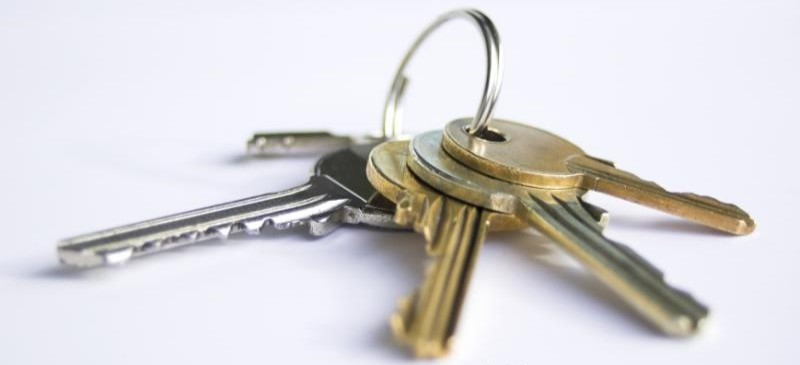
\includegraphics[width=\paperwidth,height=\paperheight]{img/the-keys-to.jpg}
}
\begin{frame}
\end{frame}
}



\begin{frame}{¿Qu\'e es una llave candidata?}
    \begin{block}<2>{Llave candidata}
        Un conjunto de uno o m\'as atributos $K = \{A_1,A_2,...,A_n\}$ es una llave candidata
        de la relaci\'on $R$ si cumple las siguiente propiedades:
        \begin{enumerate}
            \item \textbf{Unicidad}: En cualquier momento dado, no existen dos tuplas
            distintas de $R$ con los mismos valores para $A_1,A_2,...,A_n$.
            \item \textbf{Minimalidad}: Ning\'un subconjunto propio de $K$ tiene la
            propiedad de unicidad.
        \end{enumerate}
    \end{block}
\end{frame}

\begin{frame}
    \centering
    \LARGE \textcolor{blue3}{¿Cómo encontrar las llaves candidatas de una relaci\'on?}
\end{frame}


\begin{frame}{La idea es muy f\'acil}

    Sea $U = \{A_1,...,A_n\}$ el conjunto universo de los atributos de una relaci\'on $R$,

    por cada subconjunto de atributos $X \subseteq U$ comprobar la unicidad y minimalidad.
\end{frame}

\begin{frame}{Minimalidad}
    Un conjunto $C$ es minimal con respecto a una propiedad $P$ si y s\'olo si:\begin{enumerate}
        \item $P(C)$
        \item $\not \exists C' \subset C : P(C')$
    \end{enumerate}
    \vspace{5mm}

    \centering
    \onslide<2>{\Large \textcolor{red}{ Para comprobar la minimalidad debemos comprobar la unicidad}}
\end{frame}


\begin{frame}{Unicidad}
    \centering
    \LARGE ¿Qué es la unicidad?
\end{frame}

\begin{frame}{Unicidad}
    Sea $K = \{A_1,A_2,...,A_n\}$ un conjunto de atributos de
    una relaci\'on $R$, en cualquier momento dado, no existen dos tuplas
    distintas de $R$ con los mismos valores para $A_1,A_2,...,A_n$.
    \vspace{4mm}

    \onslide<2>{
    \centering
    \begin{tikzpicture}
        \node at (0,2) {LLAVE};
        \draw (0,0) node[ellipse, minimum height=3cm,minimum width=2.4cm,draw] {};
        \node at (5,2) {CUERPO};
        \draw (5,0) node[ellipse, minimum height=3cm,minimum width=2.4cm,draw] {};

        \node[circle,fill=black, inner sep=2pt] (k1) at (0,1) {};
        \node[circle,fill=black, inner sep=2pt] (k2) at (0.5,0.5) {};
        \node[circle,fill=black, inner sep=2pt] (k3) at (0,0) {};
        \node[circle,fill=black, inner sep=2pt] (k4) at (0.5,-0.5) {};
        \node[circle,fill=black, inner sep=2pt] (k5) at (0,-1) {};

        \node[circle,fill=black, inner sep=2pt] (p1) at (5,1) {};
        \node[circle,fill=black, inner sep=2pt] (p2) at (4.5,0.5) {};
        \node[circle,fill=black, inner sep=2pt] (p3) at (5,0) {};
        \node[circle,fill=black, inner sep=2pt] (p4) at (4.5,-0.5) {};
        \node[circle,fill=black, inner sep=2pt] (p5) at (5,-1) {};

        \draw (k1) -- (p1);
        \draw (k2) -- (p2);
        \draw (k3) -- (p3);
        \draw (k4) -- (p4);
        \draw (k5) -- (p5);

        
      
    \end{tikzpicture}
    }
\end{frame}


\begin{frame}{Unicidad}
    Sea $K = \{A_1,A_2,...,A_n\}$ un conjunto de atributos de
    una relaci\'on $R$, en cualquier momento dado, no existen dos tuplas
    distintas de $R$ con los mismos valores para $A_1,A_2,...,A_n$.
    \vspace{4mm}

    \centering
    \begin{tikzpicture}
        \node at (0,2) {LLAVE};
        \draw (0,0) node[ellipse, minimum height=3cm,minimum width=2.4cm,draw] {};
        \node at (5,2) {CUERPO};
        \draw (5,0) node[ellipse, minimum height=3cm,minimum width=2.4cm,draw] {};

        \node[circle,fill=black, inner sep=2pt] (k1) at (0,1) {};
        \node[circle,fill=black, inner sep=2pt] (k2) at (0.5,0.5) {};
        \node[circle,fill=black, inner sep=2pt] (k3) at (0,0) {};
        \node[circle,fill=black, inner sep=2pt] (k4) at (0.5,-0.5) {};
        \node[circle,fill=black, inner sep=2pt] (k5) at (0,-1) {};

        \node[circle,fill=black, inner sep=2pt] (p1) at (5,1) {};
        \node[circle,fill=black, inner sep=2pt] (p2) at (4.5,0.5) {};
        \node[circle,fill=black, inner sep=2pt] (p3) at (5,0) {};
        \node[circle,fill=black, inner sep=2pt] (p4) at (4.5,-0.5) {};


        \draw (k1) -- (p1);
        \draw (k2) -- (p2);
        \draw (k3) -- (p3);
        \draw (k4) -- (p4);
        \draw[color=red] (k5) -- (p4);

        
      
    \end{tikzpicture}
    

    \vspace{3mm}

    \centering
    \Large \textcolor{red}{No necesariamente es una funci\'on inyectiva}

    \note{@NOTE destacar q puede haber varias llaves candidatas a primaria}
\end{frame}






\begin{frame}{¿Esta definici\'on ayuda a obtener un algoritmo?}
    Determinar la existencia de una funci\'on entre dos conjuntos de elementos desconocidos
    
    \vspace{5mm}

    \onslide<2>{
        \centering
        \Large \textcolor{red}{¿C\'omo podemos hacer esto?}
    }
\end{frame}


\begin{frame}{Ya sabemos que existen algunas}
    \begin{itemize}
        \item Los proveedores de correo (Google, Yahoo, Outlook, etc.) asocian al
        correo algunos datos personales como el nombre y apellido.
        \item Existe un convenio internacional en el que los pa\'ises acuerdan c\'odigos para
        identificar la ubicaci\'on geogr\'afica (c\'odigo postal).
    \end{itemize}
    \vspace{5mm}

    \onslide<2>{

        Si se desea desarrollar un sistema que requiera tanto los datos personales como la
        ubicaci\'on geogr\'afica del usuario, cu\'al ser\'ia la llave primaria de la relaci\'on Usuario.
    }

\end{frame}


\begin{frame}{Buscando una llave candidata}
    \centering
    \textbf{Usuario}(Email, Nombre, Apellido, C. Postal, Provincia, Pa\'is)
    \vspace{5mm}
    
    \begin{itemize}
        \item<2->  Si conocemos el email de un usuario tambi\'en conocemos su nombre y apellido.
        $$
        \textnormal{Email} \to \textnormal{Nombre, Apellido}
        $$
        \item<3->  Si conocemos el c\'odigo postal de un usuario tambi\'en conocemos su provincia y pa\'is.
        $$
        \textnormal{C. Postal} \to \textnormal{Provincia, Pa\'is}
        $$
    \end{itemize}
    \vspace{5mm}
    
    \onslide<4>{

        \Large \textcolor{red}{¿Cu\'al ser\'ia una llave candidata de esta relaci\'on?}
    }
\end{frame}

\begin{frame}{¿Y si componemos las funciones que ya conocemos?}

    $$
        \textnormal{Email, C. Postal} \to \textnormal{Nombre, Apellido, Provincia, Pa\'is}
    $$
    \vspace{2mm}

    \onslide<2->{

        \begin{itemize}
            \item Supongamos un usuario con email luis.fonseca@gmail.com
            $$
                \textnormal{luis.fonseca@gmail.com} \to \textnormal{Luis, Fonseca}
            $$
            \item Supongamos que tiene el c\'odigo zip 10400
            $$
                \textnormal{10400} \to \textnormal{La Habana, Cuba}
            $$
        \end{itemize}
    }

    \onslide<3>{

        $$\textnormal{luis.fonseca@gmail.com, 10400} \to \textnormal{Luis, Fonseca, La Habana, Cuba}$$
    }

\end{frame}


% \begin{frame}{¿Y si componemos las funciones que ya conocemos?}

%     $$
%         \textnormal{Email, C. Postal} \to \textnormal{Nombre, Apellido, Provincia, Pa\'is}
%     $$
%     \vspace{2mm}

%     \begin{itemize}
%         \item Supongamos un usuario con email luis.fonseca@gmail.com
%         $$
%             \textnormal{luis.fonseca@gmail.com} \to \textnormal{Luis, Fonseca}
%         $$
%         \item Supongamos que tiene el c\'odigo zip 10400
%         $$
%             \textnormal{10400} \to \textnormal{La Habana, Cuba}
%         $$
%     \end{itemize}

    
%     $$\textnormal{luis.fonseca@gmail.com, 10400} \to \textnormal{Luis, Fonseca, La Habana, Cuba}$$

% \end{frame}


\begin{frame}{Dependencia Funcional}
  

    Dada una relaci\'on $R$ y los atributos $X$, $Y$ de $R$, se dice que $Y$ depende funcionalmente de $X$ si
    y s\'olo si el valor de $X$ en cada tupla de $R$ determina el valor
    de $Y$ en dicha tupla. Se representa como $R.X \to R.Y$ o simplemente

    \begin{Huge}
        
        $$
            X \to Y
        $$
    \end{Huge}

    \begin{block}{Notaci\'on}
        \begin{itemize}
            \item Atributo simple: $A,B,C,D,E$
            \item Atributo compuesto (conjunto de atributos simples): $W,X,Y,Z$
        \end{itemize}
    \end{block}
\end{frame}


\begin{frame}{Cumplimiento de una Dependencia Funcional}
    \begin{columns} 
        \column{0.5\textwidth}
        \begin{block}<2->{Funci\'on $f$}
            $$
            x_1 = x_2 \implies f(x_1) = f(x_2)
            $$
        \end{block}
        \begin{block}<3->{Dependencia Funcional $X \to Y$}
            $$
            t_1[X] = t_2[X] \implies t_1[Y] = t_2[Y] 
            $$
        \end{block}

        \column{0.5\textwidth}
        \centering
        \only<4->{
        \begin{tabular}{|c|c|c|}
            \hline
            \underline{\#E} & Grupo & Provincia \\[1mm]
            \hline
            1 & 211 & Pinar del R\'io \\
            2 & \textcolor<8->{red}{212} & \textcolor<8->{red}{La Habana} \\
            3 & \textcolor<8->{red}{213} & \textcolor<8->{red}{La Habana} \\
            15 & 211 & Pinar del R\'io \\
            \hline
        \end{tabular}
        }
        \vspace{5mm}

        \begin{itemize}
            \item<5-> \#E $\to$ Grupo, Provincia
            \item<6-> Grupo $\to$ Provincia
        \end{itemize}
        \vspace{5mm}

        \only<7->{\textcolor{red}{?`Provincia $\to$ Grupo?}}
    \end{columns}
    % Sean 
    % $U = A_1,...,A_n$ el universo de atributos de la
    % relaci\'on $R$, $X \subseteq U$ y $Y \subseteq U$. La dependencia
    % funcional $X \to Y$ se cumple en $R$ si para toda instancia $r(R)$ para todos
    % los pares de tuplas $t_1$ y $t_2$ en $r$ se cumple que:

    % $$
    %     t_1[X] = t_2[X] \implies t_1[Y] = t_2[Y] 
    % $$

    \note<1>{@NOTE ?`qu\'e es lo esencial de las funciones?}
\end{frame}

\begin{frame}{¿C\'omo representar una relaci\'on?}
    \begin{block}{Esquema relacional}
        Un \textbf{esquema relacional} expresado por $R(U,F)$
        constituye una manera abreviada de representar
        la descripci\'on de una relaci\'on mediante: 
        \begin{itemize}
            \item Su nombre $R$.
            \item El conjunto de atributos que la componen $U$, denominado universo de la relaci\'on.
            \item El conjunto de dependencias funcionales $F$ que se cumple en $R$.
        \end{itemize}
    \end{block}
    
    \note{@NOTE funciones entre los datos}
\end{frame}

\begin{frame}{Utilidad de las dependencias funcionales}
    \begin{itemize}
        \item<1-> Especificar las restricciones en el conjunto de instancias
        legales de una relaci\'on $R$ 
        (instancias $r$ de $R$ que satisfacen un conjunto de dependencias funcionales $F$):\\ 
        \centering \textcolor{red}{F se cumple en R}\vspace{2mm}
        \item<2-> Probar si una instancia $r$ de una relaci\'on $R$ es legal bajo un conjunto de
        dependencias funcionales $F$:\\
        \centering \textcolor{red}{r satisface a F} \vspace{2mm}
        \item<3-> ¿Y los algoritmos?
    \end{itemize}

    \note<2>{@NOTE hacer \'enfasis en la 2da q es la q + le interesa a ellos, pa saber si lo q existe esta' bien representado}
\end{frame}

{
\setbeamertemplate{background} 
{
    
\includegraphics[width=\paperwidth,height=\paperheight]{img/automate.jpg}
}
\begin{frame}
\end{frame}
}





\begin{frame}{Ejemplo de aplicaci\'on del algoritmo para comprobar la unicidad}
    Sea $R(U,F)$ con:
    \begin{itemize}
        \item $U = \{A,B,C,D,E,G\}$
        \item $F = \{AB \to C, {\color<3>{red}C} \to A, BC \to D, {\color<5>{red}ACD} \to B, {\color<7>{red}D} \to EG, BE \to C \}$
    \end{itemize}
    comprobar si $CD$ cumple la unicidad.
    \vspace{4mm}
    
    \onslide<2->{

        Inicializamos $X_0 = {\color<3>{red}C}D$
        \begin{enumerate}
            \item<4-> $X_1 = {\color<5>{red}ACD}$
            \item<6-> $X_2 = ABC{\color<7>{red}D}$
            \item<8-> $X_3 = ABCDEG$
        \end{enumerate}
        \onslide<9>{$X_3 = U$, se cumple la unicidad} 
    }
\end{frame}


\begin{frame}{Formalizando}

    \begin{block}{Implicaci\'on l\'ogica}
        Sea un esquema relacional $R(U,F)$ y $X \to Y$ una dependencia funcional. Se dice
        que $F$ implica l\'ogicamente a $X \to Y$ o que $X \to Y$ se
        deduce l\'ogicamente de $F$ si cada instancia $r$ de $R$ que
        satisfaga las dependencias funcionales en $F$ tambi\'en satisface $X \to Y$.

        $$
            F \models X \to Y
        $$
    \end{block}

\end{frame}


\begin{frame}{Clausura de un conjunto de atributos}
    Sea un esquema relacional $R(U,F)$, un conjunto de atributos
    $X$ tal que $X \subseteq U$.
    La clausura del conjunto de atributos $X$ con respecto a un conjunto
    de dependencias funcionales $F$ -- denotada por $X^+_F$ o abreviadamente $X^+$--
    es el conjunto de atributos simples que se determina funcionalmente por $X$ a partir
    de las dependencias funcionales de $F$.

    $$
        X^+_F = \{ A_i \in U \;|\; F \models X \to A_i\}
    $$
\end{frame}


\begin{frame}{Mejorando la definici\'on de llave candidata}
    Sea $K$ un conjunto de atributos $\{A_1, A_2, ..., A_n\}$ de una esquema
    relacional $R(U,F)$ es llave candidata candidata del esquema
    si cumple las siguientes propiedades:
    \begin{enumerate}
        \item \textbf{Unicidad}: $K^+_F = U$
        \item \textbf{Minimalidad}: Ning\'un subconjunto propio de $K$ tiene la propiedad de unicidad.
    \end{enumerate}
    
    
\end{frame}

\begin{frame}{Mejorando el algoritmo para comprobar la unicidad}

    El conjunto de atributos $X$ cumple la unicidad en $R(U,F)$ si y s\'olo si $X^+_F = U$ 
\end{frame}


\begin{frame}{¿Qu\'e herramientas podemos aplicar para inferir l\'ogicamente?}
    \onslide<2>{
        
        \begin{block}{Axiomas de Inferencia (Armstrong, 1974)}
            Sea un esquema relacional $R(U,F)$:
            \begin{enumerate}
                \item \textbf{Reflexividad}: Si $Y \subseteq X \subseteq U$, entonces $X \to Y$
                se deduce l\'ogicamente de $F$.
                \item \textbf{Aumentatividad}: Si se cumple que $X \to Y$ y $Z \subseteq U$, entonces
                $XZ \to YZ$.
                \item \textbf{Transitividad}: Si se cumple que $X \to Y$ y $Y \to Z$, entonces $X \to Z$. 
            \end{enumerate}
    
        \end{block}
        \vspace{5mm}
    
        \begin{footnotesize}
            Armstrong, W. W. [1974]. \textit{``Dependency structures of data base relationships,''}\\
            Proc. 1974 IFIP Congress, pp. 580-583, North Holland, Amsterdam.
        \end{footnotesize}
    }
\end{frame}

\begin{frame}{Lemas derivados}
    Sea un esquema relacional $R(U,F)$:
    \begin{enumerate}
        \item \textbf{Composici\'on}: $\{X \to Y, W \to Z \;|\; W \subseteq X\} \models X \to YZ$ 
        \item \textbf{Descomposici\'on}: $\{X \to Y, Z \subseteq Y\} \models X \to Z$
        \item \textbf{Pseudotransitividad}: $\{ X \to Y, WY \to Z \}  \models XW \to Z$
    \end{enumerate}
\end{frame}


\begin{frame}{Clausura de un conjunto de dependencias funcionales}
    Sea un esquema relacional $R(U,F)$. La clausura del conjunto
    de dependencias $F$ \\ -- denotada por $F^+$ -- es el conjunto de las
    dependencias funcionales implicadas l\'ogicamente por $F$. Formalmente,
    se define como:
    
    $$
        F^+=\{ X \to Y \;|\; F \models X \to Y \}
    $$

    \note{@NOTE llamar la atenci\'on sobre la dif entre $X->Y \in F$ y $F \models X->Y$ }
\end{frame}


\begin{frame}{Trivialidad de una dependencia funcional}    
    Sean $X$ y $Y$ atributos no necesariamente simples, tal que $X \cap Y = \emptyset$.\\[5mm]

    \begin{columns}[t]
        \column{.35\textwidth}
        \centering
        \only<2->{
            $X \to X$

        Trivial}

        \column{.3\textwidth}
        \centering
        \only<3->{$X \to XY$

        No trivial}

        \column{.35\textwidth}
        \centering
        \only<4->{$X \to Y$

        Completamente no trivial}
    \end{columns}

    \note<2>{@NOTE destacar que las triviales son especiales y que siempre est\'an en la clausura}
\end{frame}


\begin{frame}{¿Es viable computar $F^+$?}
    \begin{center}
        \Large
        ¿Cu\'antas dependencias funcionales triviales existen en $F^+$?
    \end{center}

        \only<2->{\large R/ La cantidad de DF's triviales es \textbf{\textcolor{red}{exponencial}} con respecto a la cantidad de atributos en $U$.}

    \onslide<3>{
\begin{center}
\Large
        ¿C\'omo podemos determinar si una dependencia funcional $X \to Y$ pertenece a $F^+$?
\end{center}
    }

    \note<2>{@NOTE no es viable computar F+}
\end{frame}

\begin{frame}{Alternativa: Utilizar la clausura de un conjunto de atributos}

    \onslide<2->{

        La clausura de un conjunto de atributos es $X^+_F = \{ A_i \in U \;|\; F \models X \to A_i\}$
        \vspace{3mm}

    \begin{columns}[t]
        \column<2->{.5\textwidth}

        ¿$X \to Y$ pertenece a $F^+$?
        \begin{enumerate}
            \item Calcular $X^+_F$
            \item Comprobar que $Y \subseteq X^+_F$
        \end{enumerate}

        \column<3->{.5\textwidth}
        \begin{algorithm}[H]
            \caption*{Get $X_F^+$}
            \begin{algorithmic}[1] % The number tells where the line numbering should start
                \STATE $S = \{X\}$
                \STATE $S' = S$\label{algorithm:attribute-clausure:line:S'}
                \FOR{each $W \to Z$ in $F$}
                    \IF{$W \subseteq S$}
                        \STATE $S = S \cup Z$
                    \ENDIF
                \ENDFOR

                \IF{$S \neq S'$}
                    \STATE \textbf{goto} line \ref{algorithm:attribute-clausure:line:S'}
                \ENDIF

                \RETURN $S$
            \end{algorithmic}
        \end{algorithm}
    \end{columns}
    }

    \note{@NOTE es en los 2 sentidos: devuelve true o false si X->Y pertenece a F+}
\end{frame}

\begin{frame}{Equivalencia de conjuntos de dependencias funcionales}

    $$
        F \equiv G \Leftrightarrow F^+ = G^+
    $$

    \begin{itemize}
        \item Se debe considerar cada $X \to Y$ en $F$ y determinar si $X^+_G$ contiene
        a $Y$.
        \item Se debe considerar cada $Z \to W$ en $G$ y determinar si $Z^+_F$ contiene
        a $W$.
    \end{itemize}
\end{frame}


\begin{frame}{Si tenemos el conjunto de DFs del universo de atributos}
    \centering
    \LARGE ¿Podemos garantizar la calidad de la base de datos?
    
\end{frame}